\section{Repetition/Introduction to Simulink/QuaRC}\label{sec:prob1}
\label{text:problem1}

\subsection{PID-(re)tuning}
The pre-tuned PID showed unsatisfactory performance and was re-tuned to better serve as the stable plant for the rest of the assignement. 

If we want a table comparing the gains...
\begin{table}[hp]
	\centering
	\caption{Controller gains comparison}
	\begin{tabular}{llll}
		\hline
		Gain & Original & New \\
		\hline
		$K_{pp}$ & 93.2 & 14.0 \\
		$K_{pd}$ & 13.2 & 2.5 \\
		$K_{ei}$ & 2.3 & 2.3 \\
		$K_{ep}$ & 7.0 & 15.0 \\
		$K_{ed}$ & 10.0 & 13.0 \\
	\end{tabular}
	\label{tab:gains}
\end{table}

\subsection{Results and discussion}

Figure \ref{fig:step_response} shows the pitch and elevation response to a step input, as well as the resulting travel rate to a step pitch input.
Would be nice to have a plot of the step responses with the original gains, to compare...

\begin{figure}[hp]
	\centering
		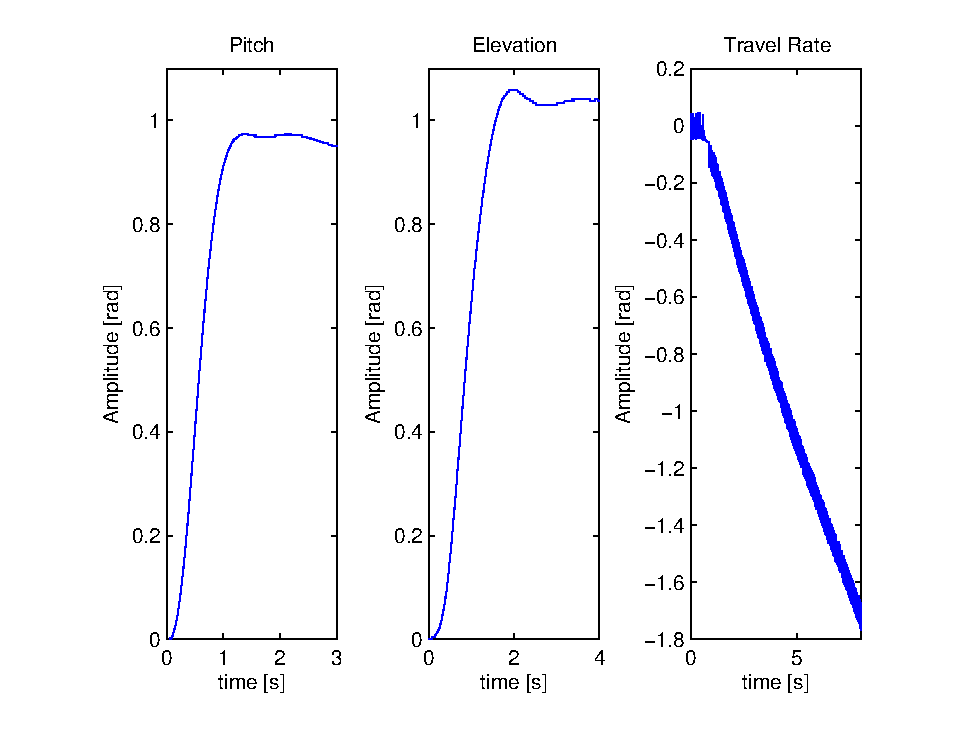
\includegraphics[width=0.9\textwidth]{figures/1/step_response.eps}
	\caption{Step response.}
	\label{fig:step_response}
\end{figure}


